\documentclass{article}[12pt]
\usepackage{color,amsmath,amssymb,graphicx,fancyhdr,amsfonts,amsthm,algorithmic,verbatim,bbold,environ}
\usepackage{hyperref}
\usepackage{mkolar_definitions}
\usepackage{multirow}
\usepackage{diagbox}
\usepackage{longtable,booktabs}
\usepackage{geometry}
\usepackage{subfigure} 
\usepackage{indentfirst} 
\usepackage[ruled,lined,boxed,linesnumbered]{algorithm2e}

\newcommand{\tightlist}{%
  \setlength{\itemsep}{0pt}\setlength{\parskip}{0pt}}


\geometry{a4paper,scale=0.8}


\title{Online-FAST: An Online Fairness Assured Service Recommendation Strategy Considering Service Capacity Constraints}

\author{Litao Zhou, Hongbo Yang, Shiwen Dong}
\date{\today}

\usepackage[hyperref=true,backend=biber,sorting=none,backref=true]{biblatex}
\addbibresource{ref.bib}

\begin{document}

\maketitle

\section{Introduction}

\subsection{Problem Background}
% 介绍相关背景
A good recommendation system is of great significance to the trade of commodity. Traditional measure of the performance of a system is recommendation accuracy. Now the fairness of algorithms is also attracting more and more attention with the wide application of recommendation systems. Today, a good recommendation system should not only learn and predict users’ preferences to items accurately, but also avoid the unfairness between different users resulting from the recommendation. 

% 形象的问题描述(举例)
Consider a service recommendation scenario with capacity constraints, we will determine how many customers can get satisfactory service quality. For example, restaurants usually have a capacity limitation representing the number of customers that can be served during meal times. If too many customers come to the restaurant during the peak hour, the supply of the restaurant can't meet the needs of so many people. Therefore, when the number of potential users exceeds the service capacity, we have to sacrifice the interests of some users by not providing them the best recommendation in exchange for the overall capacity feasibility. As a matter of fact, if the decision is too premature, there will be great unfairness. How to ensure the fairness of recommendation while maintaining users’ actual experience is a problem we try to cope with. Unlike accuracy, which can be quantified clearly, fairness is abstract and relatively difficult to define. 

\subsection{Related Work}
Currently, researchers describe the fairness of a recommendation system from multiple perspectives, which can be divided into three categories considering different stakeholders \cite{Multisided}: customer-fairness, provider-fairness \cite{FER} and CP-fairness (both of customer and provider). Customer-fairness contains group fairness \cite{Group} and individual fairness \cite{Indi1}\cite{Indi2}. The former focuses on the balance between the superior groups and the disadvantaged groups, which requires that these two kinds of groups should have the same opportunities for a particular service so that recommendation results won’t be dominated by some specific group. More microscopically, on the other hand, the individual fairness emphasizes the internal consistency within the group, requiring that similar users should get similar treatment. This fairness can be embodied in the prediction accuracy or the similarity of actual recommendation results and the ideal recommendation results.




% 有关fairness、recommendation系统的论文综述
% dsw


% 简介FAST论文的成果,肯定其中提出的measure(我们也会采用),
In this paper, we will focus on the individual fairness of the customer, following the definition of the fairness in a research \cite{FAST} about the recommendation methods with the capacity constraint of services. The FAST algorithm (Fairness Assured service recommendation Strategy) proposed in that research is designed to guarantee the long term fairness of multi-round recommendations. By experimenting results on both real and synthetic data-sets, FAST has proved to be able to achieve higher fairness than other existing baseline methods. Additionally, it also maintains a reasonably high recommendation quality. 


\subsection{Motivation}
\label{section:motivation}
The significance of FAST system is that it proposes a formal metric of individual fairness under service capacity. The metric has proved to be useful when evaluating the fairness of recommendation results under capacity constraints. However, as for the optimization of that metric, the proposed algorithm has a few deficiencies that can't be ignored when it comes to practical deployment. 
% zlt
% 指出其解决算法上的不足之处(大批量、多次排序效率低、不符合实际)


The first deployment issue with the original algorithm lies in its high computational complexity. A global sorting on fairness degree is required for every assignment in order to find the user who should be given priority to in selecting services. For an online implementation, even if we can implement the sorting process with a priority queue, since the sorting is required for every assignment until the full top-N list is collected, the time required for a single user's request is still in linear proportion to the size of the user set. The computation of $O(n\log n)$ per request can be a large overhead for the server to be deployed.

Another thing to note is that the proposed algorithm can only calculate a global recommendation plan after all users' information has been gathered. However, in practice, users must come sequentially. A static recommendation may not have the desired effect in practice. In fact, from an economist's point of view, Ho\cite{adaptive_recommendation} pointed out that although recommendation quality may improve over the course of a session, the probability of user to consider and accept a given recommendation will degrade over the course of the session. Therefore, recommendations with an adaptive feature will always outstrip the static recommendations in quality. As for the fairness problem, even if the original FAST algorithm yields a better solution on the proposed recommendation quality metrics, an individual user in reality may be less likely to accept the recommendation results due to the system's response latency.


\subsection{Major Work and Contributions}
% 指出在线算法的必要性
% significance
% 和其他算法的耦合性能
% 支持分布式计算!
Considering the shortcomings of FAST algorithm above, it is necessary to put forward an online algorithm, which can better adapt to the requirements of actual deployment, improve the efficiency of processing a single request, and ensure the fairness of multi-round allocation. We will show in this paper that such an online algorithm can be constructed. In addition to effectively resolving the above problems, our online algorithm is able to support streamed computing and distributed architecture, which is very common in modern real-time recommendation systems\cite{stream_recommendation}. This is because the recommendation is dependent on heuristics rather than global sorting results. This improvement can make our algorithm better coupled with other recommendation algorithms, so as to realize the fairness of the recommendation system in a broader range of applications.

According to the theory of online algorithms\cite{borodin2005online}, an online algorithm is forced to make decisions that may later turn out not to be optimal, which is also the case in our problem, since we don't know the coming order of future users. In our work, such discrepancy is mainly introduced in the heuristic which ensures that later coming users may still have the chance to be allocated a better service. However, we will show that such a sacrifice would not result in a huge loss of overall performance. This idea will be captured by competitive analysis. We will compare our online algorithm with the original algorithm by calculating the competitive ratio in fairness metric, recommendation quality metric and convergence speed, through theoretical analysis and experiments.


% todo: structure of the paper

\section{Definitions}

In order to correctly quantify the fairness of the allocation system and effectively compare the performance of the algorithm, we will propose some formal definitions in this section. We will first clarify the notations that will be used through the paper, and then propose indicators to measure the fairness of the system and the quality of the recommended results respectively.

\subsection{Assumptions and Justifications}

We assume that there exists a recommendation algorithm that can provide a rating matrix $R$ and provide a  recommendation list $L_i$ for all users based on $R$. We also assume that there exists a capacity constraint on every service, and that the recommendation is executed with respect to rounds. At the end of every round, the capacity will be emptied.

To deal with the capacity constraint, directly filtering out the overcrowded services from the recommendation list of certain users will have a great chance to break the fairness. To solve the problem, we try to design a strategy to adjust $L$ and generate new recommendation lists $L^T$ which can make users’ recommendation as fair as possible without breaking capacity constraints while still preserving recommendation quality. The results will be in the form of a Top-N recommendation list for every user, where N is a constant and services will be ordered according to its rating matrix.

A single assignment from users to service is clearly not enough to ensure fairness, so our problem will focus on the accumulating fairness throughout multiple rounds. We also assume that our system focuses on a certain "active" user set, who are likely to participate in most of the recommendation rounds, so that the users will not vary very much through multiple rounds, ensuring the steadiness of the fairness scope. We also assume that the participated users will only come once in every round, which follows a given occurrence probability $A$. The user occurrence in the actual coming requests input into the algorithm should conform to the distribution $A$.


\subsection{Terminologies}

\newcommand{\tabincell}[2]{\begin{tabular}{@{}#1@{}}#2\end{tabular}}
\begin{table}[htbp]
    \begin{center}
    \begin{tabular}{|c|l|}
        \hline
        \textbf{Notions} & \textbf{Represents}  \\ \hline
        $S=\{s_1, s_2, \cdots, s_m\}$ & Set of recommended services.  \\ \hline
        $C=\left\{c_{1}, c_{2}, \ldots, c_{m}\right\}$ & Set of services’ capacity constraints.  \\ \hline
        $U=\left\{u_{1}, u_{2}, \ldots, u_{n}\right\}$ & Set of recommended users.  \\ \hline
        $\left\{U^{1}, U^{2}, \ldots, U^{T}\right\}$ & Set of arriving users in $T^{th}$ round.  \\ \hline
        $\left\{U_{1}, U_{2}, \ldots, U_{j}\right\}$ & \tabincell{l}{Set of  users recommended for service $j$ by the original \\ algorithm} \\ \hline
        $R=\left[r_{1,1}, r_{1,2}, \ldots, r_{n, m}\right]$ & 
        \tabincell{l}{Predicted rating matrix produced
        by the original\\  recommendation algorithm of the system;
        Each entry $r_{ij}$ \\ denotes the relevant
        rating of user $u_i$ to service $s_j$.}
  \\ \hline
        $L=\left\{l_{1}, l_{2}, \ldots, l_{n}\right\}$ & Original recommendation lists based on R.  \\ \hline
        $L^{T}=\left\{l_{1}^{T}, l_{2}^{T}, \ldots, l_{n}^{T}\right\}$
         & \tabincell{l}{Recommendation lists finally returned 
         to users in $T^{th}$ \\ round recommendation.}  \\ \hline
        $\delta^T_i$ &\tabincell{l}{
    Variable to indicate whether user $u_i$ uses
    the \\ recommendation system  in $T^{th}$ recommendation
    or not, \\where $\delta_i^T = 1$ stands for yes and $\delta_i^T = 0$  stands for no.}  \\ \hline
    \tabincell{c}{
    $Q = \left\{Q_{1}, Q_{2}, \ldots, Q_{t}\right\}$\\
    $Q_{i} = \left\{q_{i1}, q_{i2}, \ldots, q_{ij}\right\} $} & \tabincell{l} {Request Lists for every round, where $q_{ij}$ indicates \\ the user index of the  $j^{th}$ request in the $i^{th}$ round} \\ \hline
    $A = \{a_1,a_2,\ldots,a_n\}$ & The occurrence probability for user $u_i$ in a round.   \\ \hline
    \end{tabular}
    \caption{Basic Notions of Our Work}
    \label{notion}
    \end{center}
    \end{table}
    


% “虽然用了他们的定义框架和一些相同的记号,但我们研究的是不一样的问题”


The notions we'll be using are based on the framework of FAST\cite{FAST}, but with a few extra notations in order to formulate the online property. The notations are given in Table \ref{notion}.

We should note that although the measures are with respect to each big round, the input of users are not coming in a pack. Our algorithm should read $q_{ij}$ one after another and return the result without knowing any information of the later requests except for the prior probability $A$ of the users who haven't arrived yet.




\subsection{Fairness Metrics}
% 根据需要调整定义
To quantify the level of fairness, we need to formulate metrics to measure it properly. Since we consider the Top-N services, we first need to define whether 
a service is in one's Top-N sub-list.

\begin{equation}\operatorname{Is\_In}\left(s_{j}, l i s t, N\right)=\left\{\begin{array}{l}0 \text { if } s_{j} \text { is not in the top } N \text { sub-list of list } \\ 1 \text { if } s_{j} \text { is in the top } N \text { sub-list of list }\end{array}\right.\end{equation}

And we define two types of probability below to formulate a user's individual probability of receiving a service with the probability of all users.

\begin{definition}[Ideal Probability]  The probability of a service $s_{j}$ appearing in the recommendation lists of all users in $U_j = \left\{u_i | u_i \text{ owns } Q_{Tk}, \forall k \right\}$ up to $T^{t h}$ round recommendation is:
\begin{equation}
p_{j}^{T}=\frac{\sum_{u_{i} \in U_{j}} \sum_{t=0}^{T} \delta_{i}^{t} \cdot  \operatorname{Is\_In}\left(s_{j}, l_{i}^{t}, N\right)}{\sum_{u_{i} \in U_{j}} \sum_{t=0}^{T} \delta_{i}^{t}}
\end{equation}
where $\delta_{i}^{t}$ indicates the possibility that user $i$ is the owner of a request in the $t^{\text{th}}$ round.

% question: sum to average or average to sum when counting probability


\end{definition}
\begin{definition}[Actual Probability] The probability of a service $s_{j}$ appearing in the recommendation lists of user $u_{i}$ up to $T^{{th}}$ request recommendation in $Q$ is:
\begin{equation}
p_{i, j}^{T}=\frac{\sum_{t=0}^{T} \delta_{i}^{t} \cdot \operatorname{Is\_In}\left(s_{j}, l_{i}^{t}, N\right)}{\sum_{t=0}^{T} \delta_{i}^{t}}
\end{equation}
where $\delta_{i}^{t}$ indicates the possibility that user $i$ is the owner of a request in the $t^{\text{th}}$ round.
\end{definition}

Simply speaking, the Ideal Probability describes an ``average''
while the Actual Probability is of individuals.
Also notice that
if $u_i$ gets fair recommendation on $s_j$, the actual and ideal possibilities
for $s_j$ to appear in the top-N list of $u_i$ are equal.
Conversely, we can define the difference between them to be 
a measure for (un)fairness.
\begin{definition}[Service Fairness Degree]
Fairness degree of user $u_{i}$ on service $s_{j}$ up to $T^{t h}$ round recommendation:
\begin{equation}
F_{i, j}^{T}=\frac{p_{i, j}^{T}-p_{j}^{T}}{p_{j}^{T}}
\label{eqn:def_fairness}
\end{equation}
\end{definition}
This definition gives a metric for fairness. The larger $|F|$ is,
the less fairness the recommendation has.
If $F_{i, j}^{T}$ is greater than zero, it means service $s_{j}$ is allocated to $u_{i}$ 's recommendation lists more frequently than others in $U_{j} ;$ If $F_{i, j}^{T}$ is less than zero, service $s_{j}$ appears in his recommendation lists with fewer opportunities than others; If $F_{i, j}^{T}$ is equal to zero, it means $u_{i}$ gets fair recommendation on $s_{j}$.
Then for all top-N services, we can give another definition to show the fairness just among users.
\begin{definition}[Top-N Overall Fairness Degree]
Overall fairness degree of user $u_{i}$ up to $T^{t h}$ round recommendation:
\begin{equation}
F_{i}^{T}=\sum_{s_{j} \in l(N)_{i}} F_{i, j}^{T}
\end{equation}
\end{definition}
% With the measure of fairness, we can represent three levels of fairness in a formalized way:
% (1) Perfect fairness: $\forall u_{i} \in U$ and $\forall s_{j} \in l(N)_{i}, F_{i, j}^{T}=0$
% (2) Individual fairness: $\forall u_{i} \in U, F_{i}^{T}=0$.
% (3) Relative fairness: $\forall u_{i}, u_{j} \in U, F_{i}^{T}=F_{j}^{T}$

As has been argued in the FAST system\cite{FAST}, in the fairest case, the variance of Top-N fairness among users should be equal to zero, where all users have the same actual probability in receiving a service. It is also valid to take the variance among users’ Top -N Fairness $D(F_i^T)$ as a measure of the fairness of recommending system, because $F_i^T$ exactly captures the notion of the accumulating extent of a user's fairness throughout multiple rounds. The smaller the variance is, the more
fairness a recommending system has.


\subsection{Recommendation Quality Metrics}
Recap that L is the list generated by a conventional recommending algorithm, 
and $L^T$ is generated by the one which takes fairness into consideration.
Notice that the quality of recommendations may decrease due to our work to improve fairness.Since we also hope to maintain the quality while improving fairness, we should also introduce a measure for recommending quality.

%n
We only consider the quality of $l(N)_{i}$, namely the top-N list. In the new list $l_{i}^{T},$ the quality declines when a service is removed, 
and we use the service predicted rating score to measure the extent of the decline.
%r:打分
Therefore, the quality of a new recommendation list $l_{i}^{T}$ will be the sum of rating scores of all the services belonging to $l(N)_{i}$ and $l_{i}^{T}$ at the same time. 
%分母,归一化
Notice that users may give their rating in some inclination, we should make a normalization to eliminate this noise factor.

We use the highest rating of $l(N)_{i}$ as the denominator to normalize the quality score. The positions of services $p_{i, j}^{T}$ in their recommendation lists also reflect their importance to a user.($p_{i, j}^{T}$ is not possibility) The quality measurement can be extended by giving each service a logarithmic discount based on its position in $l(N)_{i} .$ The quality of recommendation lists of the entire system consists of the recommendation list quality of each user by adding them all.

\begin{definition}[Quality of Recommendation List]
Quality of outputted recommendation list $l_{i}^{T}$ of user $u_{i}$ on $T^{\text {th }}$ round recommendation:
\begin{equation}
    q_{i}^{T}=\frac{\sum_{s_{j} \in l(N)_{i} \cap l(N)_{i}^{t}} \frac{r_{i, j}}{\log _{2}\left(p_{i, j}^{T}+1\right)}}{r_{i, l(N)_{i}[0]}}
\end{equation}
where $l(N)_{i}[0]$ represents the subscript index of the service appearing at the top position of $l(N)_{i},$ and $p_{i, j}^{T}$ is the position of service $s_{j}$ in $l(N)_{i}$
\end{definition}





\section{Problem Formulation}

Based on the previous metrics, we can get the formal definition of fairness assured online recommendation problem for services with capacity constraints.

\begin{definition}[Fairness Assured Recommendation Online Problem for Services with Capacity Constraints.]

\textbf{Given}, Relevance rating matrix $R$ and original recommendation lists $\{L\}$ generated by a conventional recommendation algorithm, the set of services' capacity constraint $C$, a positive integer $N$, an set of ordered lists of recommendation requests $Q$ where $q_{ij}$ is from a set of users $U$, indicating the $j^{\text{th}}$ request in $i^{\text{th}}$ round. 


\textbf{Objective}, Finding a top-$N$ recommendation list for each request to minimize $D(F_i^T)$, where $D\left(F_{i}^{T}\right)$ represents the variance among Top-N Fairness of all users.

\textbf{Constraint},
\begin{enumerate}\setlength{\itemsep}{-0.1cm}
    \item Capacity: keeping $\forall c_{j} \in C, c_{j} \geqslant \sum_{u_{i} \in U} \delta_{i}^{T} \cdot  \operatorname{Is\_In}\left(s_{j}, l_{i}^{T}, N\right)$
    \item Recommendation Quality: preserving $\sum_{u_{i} \in U} q_{i}^{T}$ at a high level
    \item Online Property: The recommendation for $q_{ij}$ should not be affected by $q_{i'j'}$ where $ i' > i$ or  $j'> j \And i' = i$ .
\end{enumerate}

\end{definition}

The improvement in our formulation compared with the original FAST system is that our problem regulates that the requests should be taken sequentially. Our problem also takes a user coming probability $A$ instead of the fixed user set as input. These two differences are what we believe to be of the greatest help for online implementation.



%%%%%%%%%%%%%%%%%%%%%%%%%%%%%%%%%%%%%%%%%%%%%%%%%%%%%%%%%%%%
%\section{Proposed Solutions}

% 伪代码介绍在线算法

% 难点:
% 如何设计恢复机制确保Fairness指数在在线过程中依然保持valid + 证明
% 通过实验说明在线算法和quality、fairness的变化规律
% 分析新算法的时间复杂度,以及和表现的关系
% 证明在线算法的N-迭代收敛速度

What we expect to do in this project is listed as follows.
\begin{enumerate}
    \item First, we will design a heuristic to be used in the online algorithm, which will exploit the current fairness degree, service capacity distribution and the user-coming prior probability, in order to make sure that the online algorithm will still make improvements towards fairness while maintaining the recommendation quality every round.
    \item Next, we will try to prove the convergence of our algorithm in making the variance of overall fairness degree minimal.
    \item We will carry out several experiments on both real and synthetic data-sets. First, we will fix the user set, assuming that the arriving probability is $100\%$ for every user  and compare the results with the original algorithm as an initial validation.
    \item Then we try to introduce the parameter $A$ which represent the possibility user $u_i$ uses the recommendation system in each round. The experiment results will be compared with integer linear programming that only tries to maximize recommendation quality regardless of fairness, together with the random algorithm that may converge slower in fairness. The experiments may help further validate our conclusions.
\end{enumerate}

The main challenges of our work are listed as follows.

\begin{enumerate}
    \item In our on-line algorithm, each round the elements of one sub-list in the input $Q$ is treated one by one, we use heuristics to determine whether a service should be allocated to a user along with the update of $Top-N$ Fairness. We must design some recovery mechanism to ensure that fairness index remains valid at every assignment throughout the online processes.
    \item Our recommendation is dependent on heuristics rather than global sorting results, and because of the heuristics is related to $A$ , we don't know the coming users and their order in the future, which may lead to some decisions that not really optimal, but ensures that users still have the chance to get a better service. And our main efforts will lie in showing that our on-line algorithm can gain the convergence with iteration.
\end{enumerate}
%% To be deleted when submitting %%%%%%
%%%%%%%%%%%%%%%%%%%%%%%%%%%%%%%%%%%%%%%%%%%%%%%%%%%%%%%%%%%%

\section{A Fairness Guaranteed Service Recommendation Online System (Online-FAST)}

In the original FAST system, the recommendation algorithm is shown in Algorithm \ref{alg:FAST}, which assumes that the requests from users come in groups and that the system can make use of the global information (the users participating in the round) to return a fairness guaranteed recommendation result while ensuring the recommendation quality.

\begin{algorithm}[htbp]
    \KwIn{$N$: Parameter Top-$N$;\\
    \quad $l_{1}, l_{2}, \ldots, l_{n}$: Original recommendation list of users;\\
    \quad$l(N)_{1}, l(N)_{2}, \ldots, l(N)_{n}$: Original top-$N$ recommendation list of users;\\
    \quad$R$: Rating matrix;\\
    \quad$c_{1}, c_{2}, \ldots, c_{m}$: Capacity constraints of services;\\
    \quad$U_{1}, U_{2}, \ldots, U_{m}: U_{j}$: list of all items;\\
    \quad$F_{1}^{T-1}, F_{2}^{T-1}, \ldots, F_{n}^{T-1}$: Top-N Fairness of all users up to last recommendation.}
    \KwOut{$l_{1}^{T}, l_{2}^{T}, \ldots, l_{n}^{T}$: Recommendation list for all the users in $T^{t h}$ round;}
    \BlankLine
    
    \For{time $=0 \rightarrow n \times N-1$}{
        Sort users according to $F_{i}^{T-1}$ from lowest to highest \;
        rec\_user $\leftarrow$ user with the lowest $F_{i}^{T-1}$ \;
        \For{$s_{j}$ in $l(N)_{\text{rec\_user}}$}{
            \If{$c_{j}>0$}{
                $c_{j}=c_{j}-1$ \;
                Update $F_{\text{rec\_user}}^{T-1}$ \;
            }
        }
    }
    Fill $l_{i}^{T}$ whose positions are larger than $N$ in $l_{i}$ in sequence \;
    \Return{$l_{1}^{T}, l_{2}^{T}, \ldots, l_{n}^{T}$}
    \caption{Offline Fairness Assured Service Recommendation Algorithm (FAST) for Fixed Users \label{alg:FAST}}
\end{algorithm}

As has been argued in Section \ref{section:motivation}, the need of online deployment requires that the algorithm should not depend on future requests when processing a user's request. In addition, users are allowed to appear or not appear with a certain probability in each round. In order to resolve these two requirements, we present a new algorithm Online-FAST in Algorithm \ref{alg:Online-FAST} based on the framework of FAST(Algorithm \ref{alg:FAST}).

\begin{algorithm}[htb]
    \KwIn{$N$: Parameter Top-$N$;\\
    \quad $l_{1}, l_{2}, \ldots, l_{n}$: Original recommendation list of users;\\
    \quad$l(N)_{1}, l(N)_{2}, \ldots, l(N)_{n}$: Original top- $N$ recommendation list of users;\\
    \quad$R$: Rating matrix;\\
    \quad$c_{1}, c_{2}, \ldots, c_{m}$: Capacity constraints of services;\\
    \quad$F_{1}^{T-1}, F_{2}^{T-1}, \ldots, F_{n}^{T-1}$: Top-N Fairness of all users up to last recommendation;\\
    \quad$a_{1}, a_{2}, \ldots,a_{n}$: The occurrence probability of users in $T^{th}$ round;\\
    \quad$q_{i1},\ldots,q_{ik}$: The coming request of $T^{th}$ round.
    }
    \KwOut{$l_{1}^{T}, l_{2}^{T}, \ldots, l_{n}^{T}$: Recommendation list for all the users in $T^{t h}$ round;}
    \BlankLine
    \SetKwFunction{Fcheck}{IsFeasible}
    \SetKwFunction{FMain}{OnlineFast}
    \SetKwProg{Fn}{Function}{:}{\Return {$c_{\text{rec\_service}} - 1 > \text{expected\_capacity}$}}
    \Fn{\Fcheck{rec\_service, priority\_users}}{
        \textit{expected\_capacity} $= \sum_{u\in \text{priority\_users}} a_{u} \cdot I(\textit{rec\_service} \in l(N)_u)$\; % l(N) issue?
    }
    \SetKwProg{Pn}{Function}{:}{\KwRet}
    \Pn{\FMain{}}{
        served = \{\}\;
        \ForEach{request $q_{ij} \in Q_{i}$}{
            rec\_user = $q_{ij}$.user\;
            rec\_service = $l_\text{rec\_user}[0]$\;
            \While{rec\_user's top-N list is not filled}{
                priority\_users = $\left\{ u \in U/served | F_{u}^{T-1} < F_{\text{rec\_user}}^{T} \right\}$ \;
                \If{\Fcheck{rec\_service,priority\_users}}{
                    Assign rec\_service to rec\_user \;
                    $c_{j}=c_{j}-1$ \;
                    Update $F_{\text{rec\_user}}^{T-1}$ \;
                }
                rec\_service = $l_\text{rec\_user}$.next(rec\_service)\;
            }
            send the recommendation result to user\;
            add user to served set\;
        }
    }
    \caption{Online Fairness Assured Service Recommendation Algorithm (Online-FAST) for Mutable Users with Arriving Probability \label{alg:Online-FAST}}
\end{algorithm}


In an online scenario, since we don't know the future requests, many  scheduling or recommendation systems will use the preemption strategy, which always assigns the available service to first-arriving users until the capacity of the service is full. Certainly, such strategy ensures a relatively optimal result under an online setting. However, it fails to ensures the fairness of users throughout multiple rounds. It might be the case that a large number of users' requests arrive almost at the same time. However, due to network speed, server routing, backend mechanism and other problems, they are identified as a series of successive requests by the server and are processed in an preemptive approach which should not exist.

In order to eliminate the potential unfairness risks in preemption algorithms, we need to design a strategy where those who arrive first can reserve a portion of his best services for those who need it later, and this waiver mechanism should not unduly affect the quality of the recommendation. In Online-FAST, we introduce a utility function called \texttt{IsFeasible} to determine whether the current user should be recommended or give up a service.


The \texttt{IsFeasible} function will estimate the number of users that may appear in the future, for whom assigning the services can leads to a reduce in the global difference of fairness degree, and then compare it with the capacity of the current service. It will return false if the job should not be assigned to the current user and be prepared for future users, and return true if the assignment of the service will not cause future unfairness. 

Compared to FAST, the \texttt{IsFeasible} function can be viewed as a ``smaller'' effort towards reducing unfairness since it makes an under-approximation of future unfairness. Therefore, the algorithm should converge slower than FAST. We will later show by experiments that the online-FAST can still ensure the convergence of fairness degree, and will maintain the convergence rate at a practical level.


\section{Analysis}


\subsection{Correctness}

In order to ensure the functional correctness of Online-FAST, we claim two important properties, and relevant proofs can refer to Appendix A.

\begin{theorem}[Fairness Degree Converges to Zero] Given the arriving probability $A$ for the user set, the sum of Top-N Fairness Degree of all the users in each round will approach to zero (i.e.  $\lim_{T \rightarrow \infty}\sum_{u_{i} \in U} F_{i}^{T}=0$) if and only if the users share a same arriving probability.
\label{thm1}
\end{theorem}

Theorem \ref{thm1} indicates that when considering arriving probability, the fairness degree should be calculated and maintained globally, no matter whether the user actually comes in the current round, and that the arriving probabilities for the users should be the same, otherwise our proposed fairness degree will lose the converge-to-zero property, thus failing to accurately describe the fairness of the recommendation system.

This property can be further illustrated by the two figures in \ref{fig:thm1}. We compare experiments on different strategies on users with the same arriving probability against users with diverse arriving probability. If the users have a different arriving probability, the preempt algorithm will not keep the average of fairness degree to zero.

\begin{figure}[htbp]
  \centering
  \subfigure{
    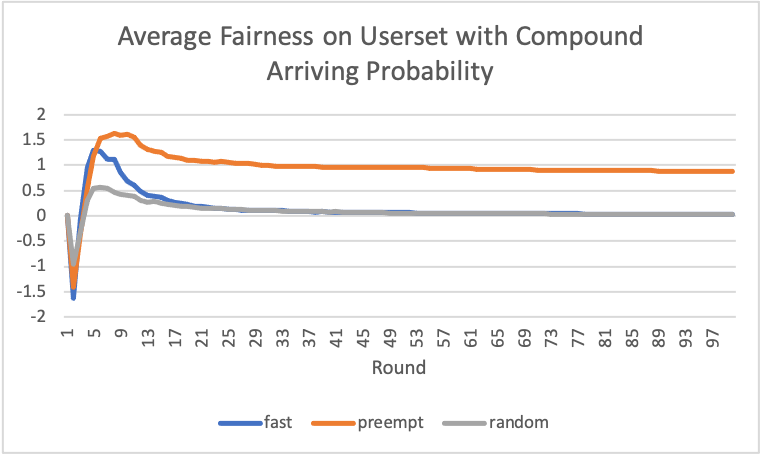
\includegraphics[scale=0.21]{img/thr1.png}}
  \hspace{0.1in} % 两图片之间的距离
  \subfigure{
    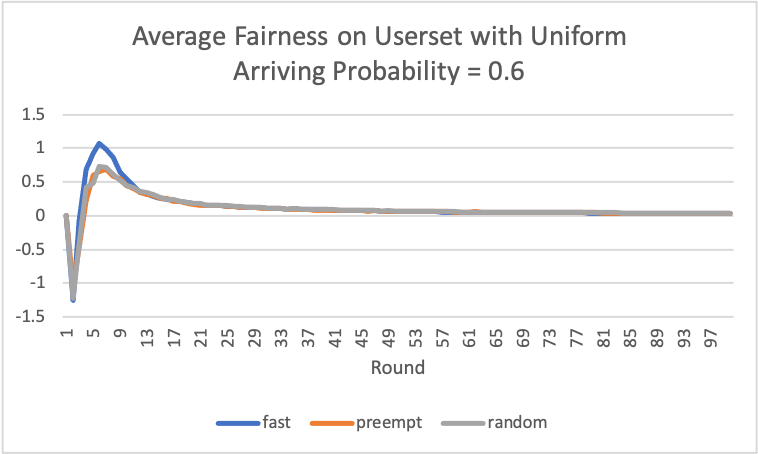
\includegraphics[scale=0.21]{img/thr2.png}}
  \caption{An intuitive interpretation of Theorem \ref{thm1}
  \label{fig:thm1}}
\end{figure}


Based on Theorem \ref{thm1}, we can argue the functional correctness of our online-FAST algorithm. Claim \ref{thm2} indicates F-FAST can assure long-term fairness for multi-round recommendations in an online scenario where users' arriving probabilities are given.


\begin{claim}[Variance Convergence] For a group of users with the same arriving probability, assume the arrival of them are uniformly distributed. The variance among the Top-N fairness of them $D\left(F_{i}^{T}\right)$ converges with the recommended round $T$.
\label{thm2}
\end{claim}

The reasoning in Claim \ref{thm2} depends heavily on the assumption that the arrival order of users conforms to uniform distribution. Furthermore, in the process of reasoning, we used some intuitive observations to reach conclusions. Therefore, we need to further illustrate the convergence of the algorithm through experiments. 

% 我们为验证算法有效性做的实验

% 介绍dataset
% Dataset的生成方式
\begin{frame}{Experiment: Dataset Preparation}
    \begin{block}{Dataset}
    \begin{enumerate}
        \item Yelp Dataset: real world dataset
        \begin{enumerate}
        \item Phoenix
        \item Toronto
        \end{enumerate}
        
        \item Synthetic dataset, generated by different param-settings
        \begin{enumerate}
        \item Dataset 1 : Slack capacity constraints 
        \item Dataset 2 : balanced capacity constraints
        \item Dataset 3 : prominent capacity conflicts 
        \item Dataset 4 : serious capacity conflicts
        \end{enumerate}
        
    \end{enumerate}
    \end{block}
    \begin{block}{Evaluation Metric}

         \begin{enumerate}
        \item Total quality of recommendations of each user
        \item Variance among Top-N Fairness of all users
        \end{enumerate}

    
        \end{block}
    
\end{frame}





% 介绍使用到对比的另两种方法
\begin{frame}{Experiment: Constrast Algorithms}
    We compare our algorithm against the following two baseline methods
    
    \begin{block}{Preempt Strategy}
A kind of first-come first-served (FCFS) process scheduling algorithm which doesn’t take fairness into consideration
    
        \end{block}
        \begin{block}{Random Strategy}
Assign Services to users randomly, which can also assure Top-N Fairness in the long run.
        \end{block}
    
\end{frame}




% 分别介绍真实数据集和人工数据集的实验情况,插入图表
\begin{frame}{Experiment on Yelp Dataset}


\begin{figure}[htbp]
\centering
\subfigure{
\begin{minipage}[t]{0.36\linewidth}
\centering
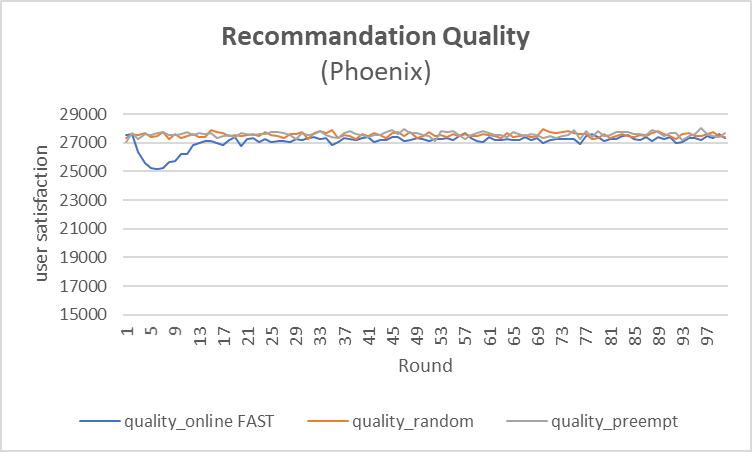
\includegraphics[width=1.6in]{img/2_q_p.png}
\end{minipage}%
}%
\subfigure{
\begin{minipage}[t]{0.36\linewidth}
\centering
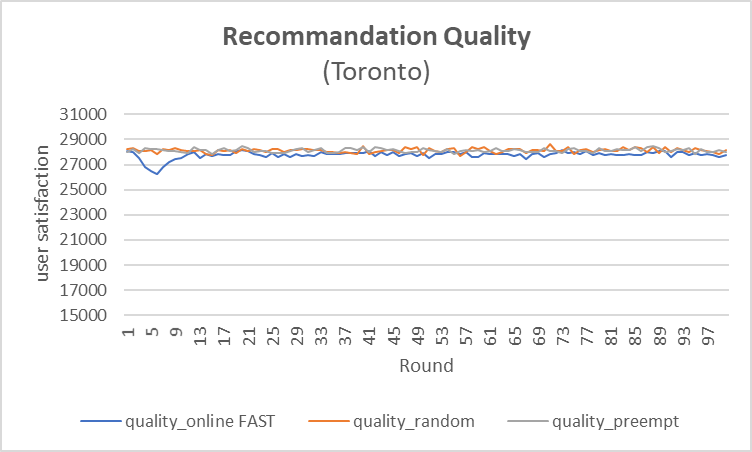
\includegraphics[width=1.6in]{img/2_q_t.png}
\end{minipage}%
}%
\caption{Online FAST keeps Recommendation Quality at a high level}
\end{figure}

\begin{figure}
\subfigure{
\begin{minipage}[t]{0.36\linewidth}
\centering
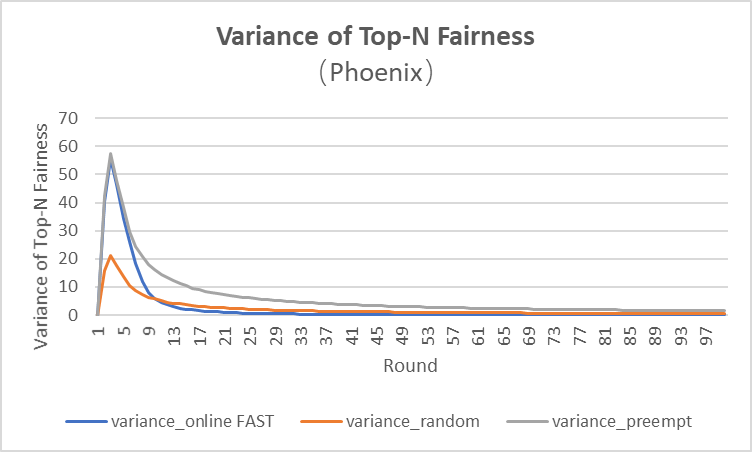
\includegraphics[width=1.6in]{img/2_v_p.png}
\end{minipage}
}%
\subfigure{
\begin{minipage}[t]{0.36\linewidth}
\centering
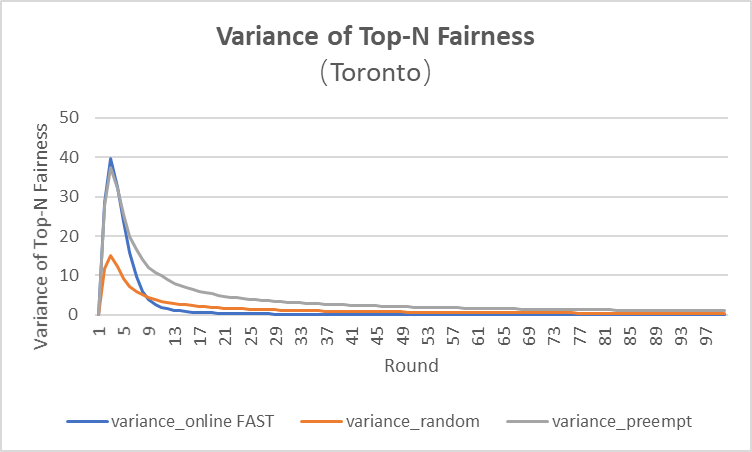
\includegraphics[width=1.6in]{img/2_v_t.png}
\end{minipage}
}%
\centering
\caption{Online FAST shows better convergence property (Arrival Probability = 0.8, N = 5)}
\end{figure}
\end{frame}


\begin{frame}{Experiment on Synthetic Dataset }

\begin{figure}[htbp]
\centering
\subfigure[Dataset 1]{
\begin{minipage}[t]{0.36\linewidth}
\centering
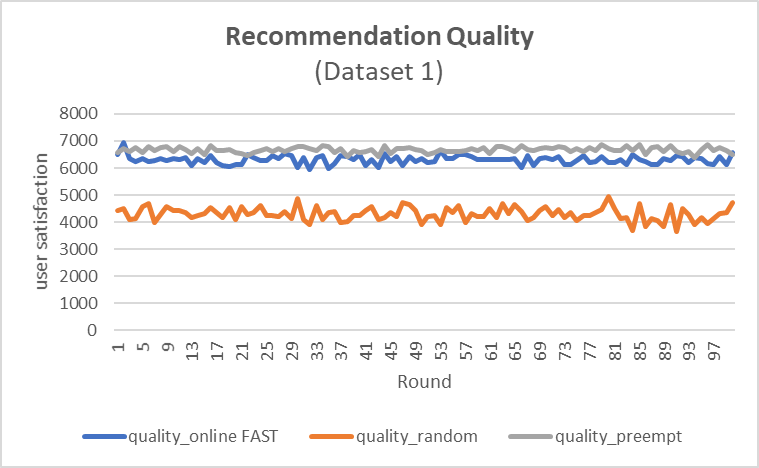
\includegraphics[width=1.6in]{img/1_q_1.png}
\end{minipage}%
}%
\subfigure[Dataset 2]{
\begin{minipage}[t]{0.36\linewidth}
\centering
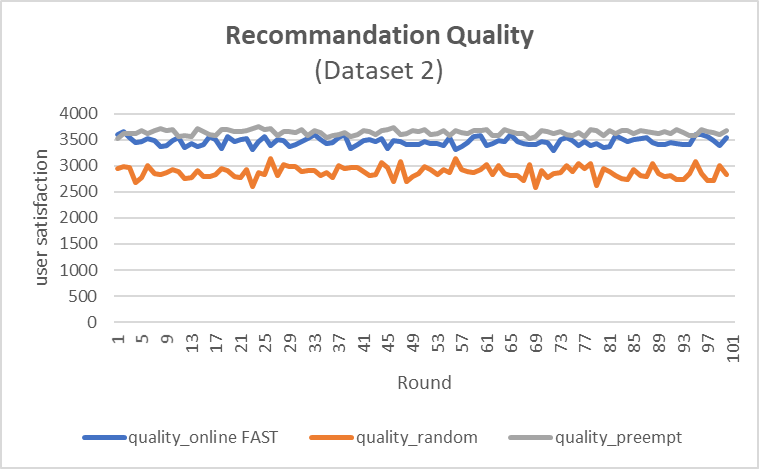
\includegraphics[width=1.6in]{img/1_q_2.png}
\end{minipage}%
}%

\subfigure[ Dataset 3]{
\begin{minipage}[t]{0.36\linewidth}
\centering
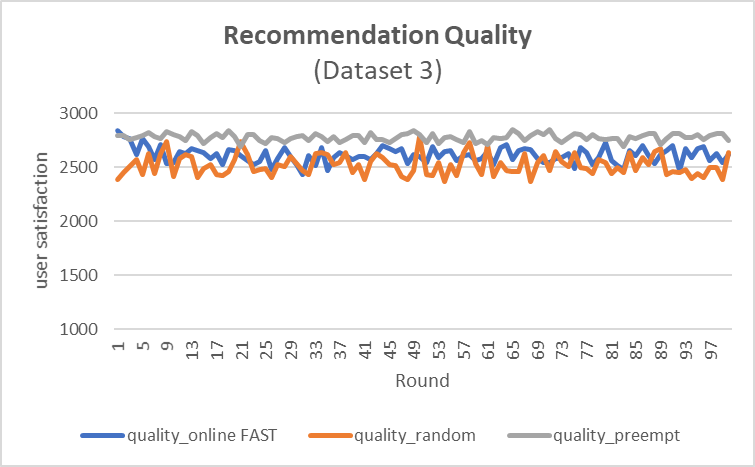
\includegraphics[width=1.6in]{img/1_q_3.png}
\end{minipage}
}%
\subfigure[Dataset 4]{
\begin{minipage}[t]{0.36\linewidth}
\centering
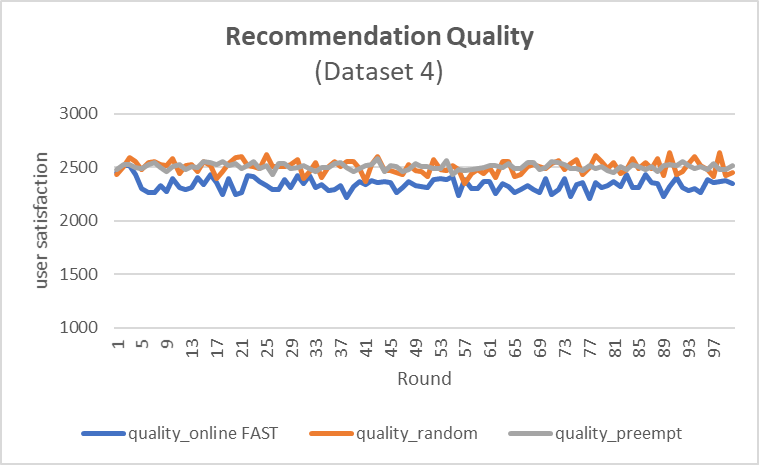
\includegraphics[width=1.6in]{img/1_q_4.png}
\end{minipage}
}%
\centering
\caption{Recommendation Quality of Online-FAST is steady under different levels of capacity constraints\ (Arrival Probability = 0.6, N = 5)}
% \label{fig:RQ}
\end{figure}
\end{frame}


\begin{frame}{Experiment on Synthetic Dataset}

\begin{figure}[htbp]
\centering
\subfigure[Dataset 1]{
\begin{minipage}[t]{0.36\linewidth}
\centering
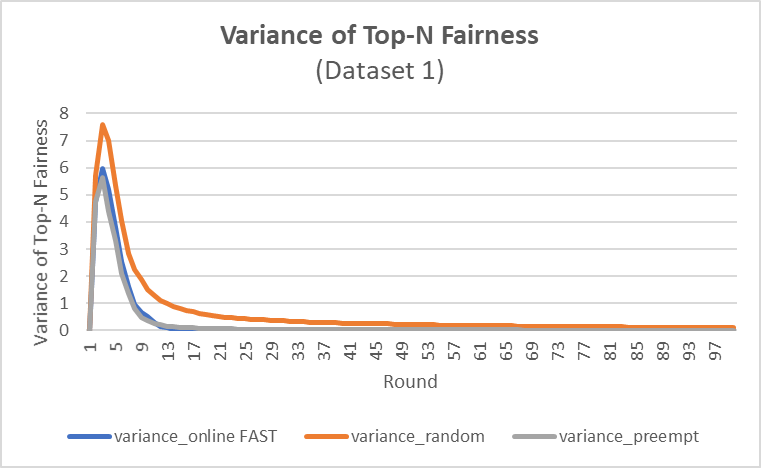
\includegraphics[width=1.6in]{img/1_v_1.png}
\end{minipage}%
}%
\subfigure[Dataset 2]{
\begin{minipage}[t]{0.36\linewidth}
\centering
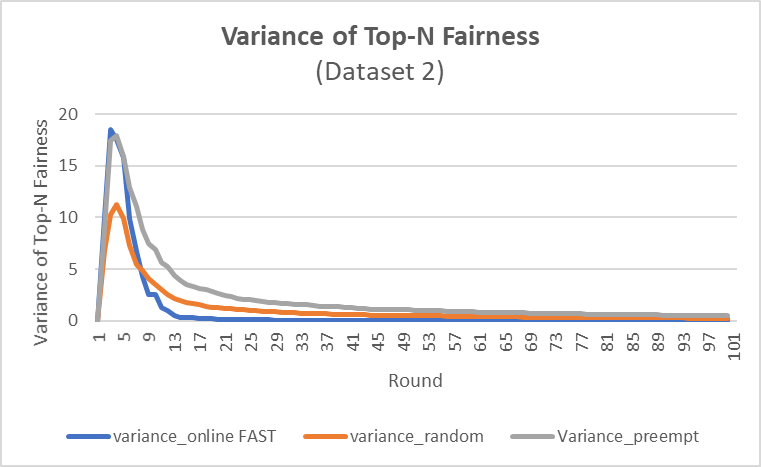
\includegraphics[width=1.6in]{img/1_v_2.png}
\end{minipage}%
}%

\subfigure[ Dataset 3]{
\begin{minipage}[t]{0.36\linewidth}
\centering
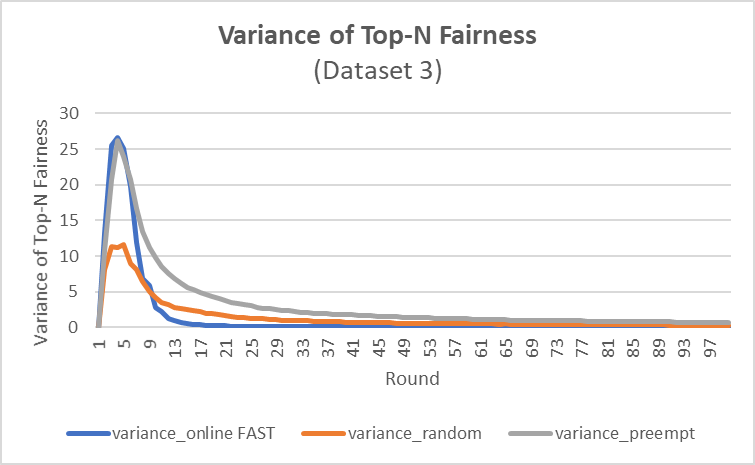
\includegraphics[width=1.6in]{img/1_v_3.png}
\end{minipage}
}%
\subfigure[Dataset 4]{
\begin{minipage}[t]{0.36\linewidth}
\centering
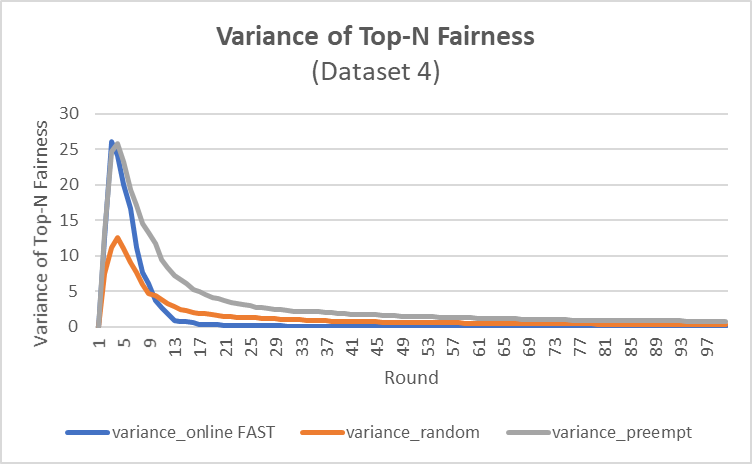
\includegraphics[width=1.6in]{img/1_v_4.png}
\end{minipage}
}%
\centering
\caption{Variance of Top-N Fairness can converge under different levels of capacity constraints (Arrival Probability = 0.6, N = 5)}
\end{figure}
\end{frame}


\begin{frame}{Experiment on Synthetic Dataset}

\begin{figure}[htbp]
\centering
\subfigure[P=0.5]{
\begin{minipage}[t]{0.36\linewidth}
\centering
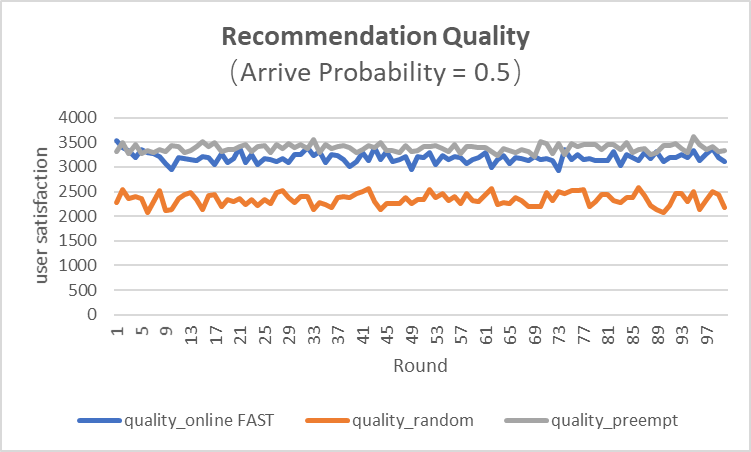
\includegraphics[width=1.6in]{img/3_q_0.5.png}
\end{minipage}%
}%
\subfigure[P=0.6]{
\begin{minipage}[t]{0.36\linewidth}
\centering
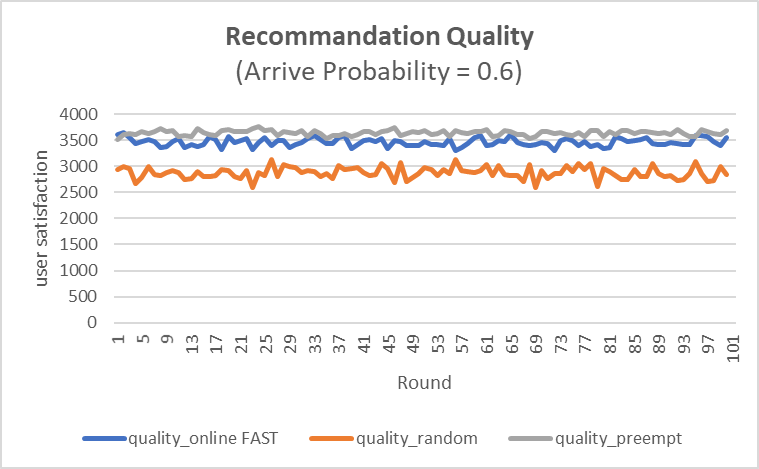
\includegraphics[width=1.6in]{img/3_q_0.6.png}
\end{minipage}%
}%

\subfigure[P=0.7]{
\begin{minipage}[t]{0.36\linewidth}
\centering
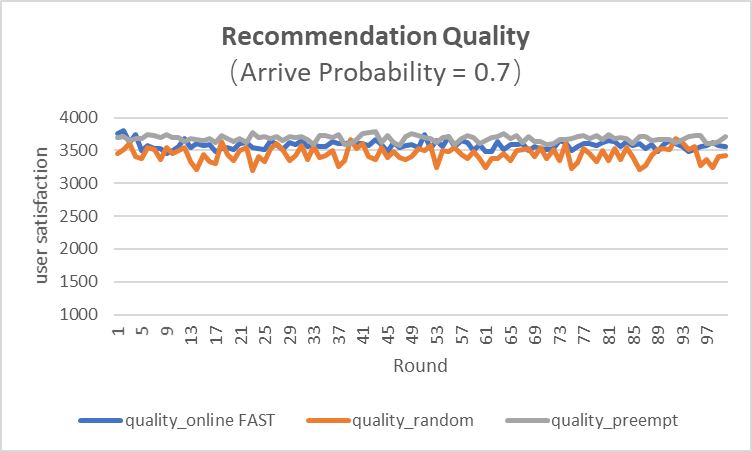
\includegraphics[width=1.6in]{img/3_q_0.7.png}
\end{minipage}
}%
\subfigure[P=0.8]{
\begin{minipage}[t]{0.36\linewidth}
\centering
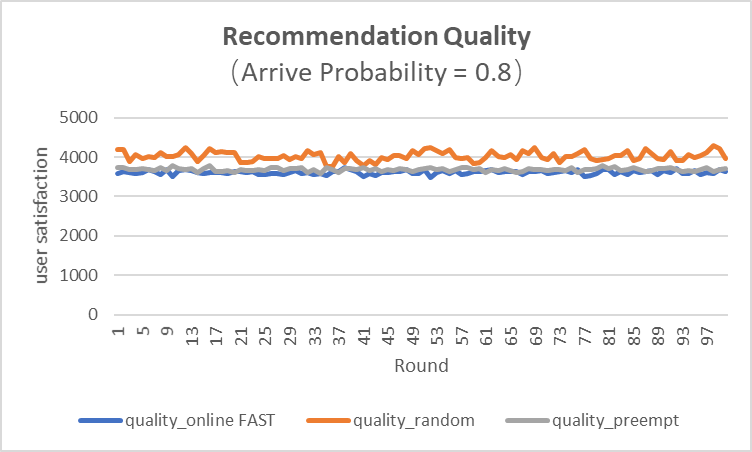
\includegraphics[width=1.6in]{img/3_q_0.8.png}
\end{minipage}
}%
\centering
\caption{Recommendation Quality is steady under different arriving probability  (on Balanced Capacity Constraints Dataset, N = 5)}
\end{figure}
\end{frame}






\section{Conclusion}

In this paper, we further expand the notion of individual fairness by improving FAST algorithm. To be specific, we first introduce user sets with arrival probability into the original FAST framework, and formally prove the soundness of fairness degree. Next, we make the FAST algorithm more suitable for online deployment by designing an online algorithm with $O(N)$ cost per request, compared with $O(N \log N)$ in Offline-FAST. Its online property will also make the decision process independent of future requests, thus making the algorithm more practical.

Through theoretical analysis and experiments, our work further enhances the practical value and application range of the fairness degree adopted in the FAST algorithm. It is shown that under dynamic user sets and online scenarios, FAST framework can still achieve the purpose of assuring the fairness among users, without losing the recommendation quality. Further work that can be done on the FAST framework includes research into user requests with dynamic arriving probability, or cases where the original recommendation algorithm gives non-uniform recommendation results in different rounds.



\appendix

\section{Proof of Properties for Online-FAST}

\textbf{Theorem 1} (Fairness Degree Converges to Zero) Given the arriving probability $A$ for the user set, the sum of Top-N Fairness Degree of all the users in each round will approach to zero (i.e.  $\lim_{T \rightarrow \infty}\sum_{u_{i} \in U} F_{i}^{T}=0$) if and only if the users share a same arriving probability.
\begin{proof}

The sum of Top-N Fairness at the $T^{th}$ round can be formulated as:
\begin{equation}
    \sum_{u_{i} \in U} F_{i}^{T}=\sum_{u_{i} \in U} \sum_{s_{j} \in l(N)_{i}} \frac{p_{i, j}^{T}-p_{j}^{T}}{p_{j}^{T}}
    \label{thm1-1}
\end{equation}

We can reformulate Equation \ref{thm1-1} as:
\begin{equation}
    \sum_{u \in U} F_{i}^{T}=\sum_{s_{j} \in S} \sum_{u_{i} \in U_{j}}\left( \frac{p_{i, j}^{T}}{p_{j}^{T}}-1\right)
    \label{thm1-2}
\end{equation}

For each addend in Equation \ref{thm1-2}, by substituting $p_{i,j}$ and $p_{j}$ with their definitions, we can get:
\begin{equation}
    \begin{aligned}
    \frac{p_{i,j}^{T}}{p_j^T} &= \frac{\frac{\sum_{t=0}^{T} \delta_{i}^{t} \cdot \operatorname{Is\_In}\left(s_{j}, l_{i}^{t}, N\right)}{\sum_{t=0}^{T} \delta_{i}^{t}}}
    {\frac{\sum_{u_{k} \in U_{j}} \sum_{t=0}^{T} \delta_{k}^{t} \cdot  \operatorname{Is\_In}\left(s_{j}, l_{k}^{t}, N\right)}{\sum_{u_{k} \in U_{j}} \sum_{t=0}^{T} \delta_{k}^{t}}} \\
    &= \frac{{\sum_{u_{k} \in U_{j}} \sum_{t=0}^{T} \delta_{k}^{t}}}{{\sum_{t=0}^{T} \delta_{i}^{t}}}
    \cdot
    \frac{{\sum_{t=0}^{T} \delta_{i}^{t} \cdot \operatorname{Is\_In}\left(s_{j}, l_{i}^{t}, N\right)}}{\sum_{u_{k} \in U_{j}} \sum_{t=0}^{T} \delta_{k}^{t} \cdot  \operatorname{Is\_In}\left(s_{j}, l_{k}^{t}, N\right)} \\
    &\stackrel{{T\rightarrow \infty}}{\longrightarrow} \frac{\sum_{u
    _k \in U_{j}} a_k }{ a_i} \cdot \frac{{\sum_{t=0}^{T} \delta_{i}^{t} \cdot \operatorname{Is\_In}\left(s_{j}, l_{i}^{t}, N\right)}}{\sum_{u_{k} \in U_{j}} \sum_{t=0}^{T} \delta_{k}^{t} \cdot  \operatorname{Is\_In}\left(s_{j}, l_{k}^{t}, N\right)} \\
    &\stackrel{{T\rightarrow \infty}}{\longrightarrow} \frac{\sum_{u
    _k \in U_{j}} a_k }{ a_i}
    \cdot
    \frac{{a_i \cdot \sum_{t=0}^{T} \operatorname{Is\_In}\left(s_{j}, l_{i}^{t}, N\right)}}{\sum_{u_{k} \in U_{j}} a_{k} \cdot  \sum_{t=0}^{T}  \operatorname{Is\_In}\left(s_{j}, l_{k}^{t}, N\right)} \\
    &= \frac{\left(\sum_{u
    _k \in U_{j}} a_k\right) \left(\cdot \sum_{t=0}^{T} \operatorname{Is\_In}\left(s_{j}, l_{i}^{t}, N\right)\right)}{\sum_{u_{k} \in U_{j}} \left(a_{k} \cdot  \sum_{t=0}^{T}  \operatorname{Is\_In}\left(s_{j}, l_{k}^{t}, N\right)\right)}
    % \frac{\sum\limits_{u_k \in U_j^T}{\sum\limits_{t=0}^{T}\delta_{k}^{t}}}{1}
    \end{aligned}
    \label{thm1-3}
\end{equation}

To make the second $\stackrel{{T\rightarrow \infty}}{\longrightarrow}$ derivation hold, we specify that $\operatorname{Is\_In}\left(s, l_{i}^{T}, N\right) = 0$ if $u_i \notin U^{T}$ for any service $s$ and list length $N$, which is compatible with the definition and the algorithm implementation.

Now we can further reformulate each addend in Equation \ref{thm1-2} as follows
\begin{equation}
    \begin{aligned}
        \sum_{u_{i} \in U_{j}}\left( \frac{p_{i, j}^{T}}{p_{j}^{T}}-1\right) 
        & \stackrel{{T\rightarrow \infty}}{\longrightarrow} \frac{\sum_{u_i \in U_j} \left(\sum_{u_k \in U_{j}} a_k\right) \left( \sum_{t=0}^{T} \operatorname{Is\_In}\left(s_{j}, l_{i}^{t}, N\right)\right)}{\sum_{u_{k} \in U_{j}} \left(a_{k} \cdot  \sum_{t=0}^{T}  \operatorname{Is\_In}\left(s_{j}, l_{k}^{t}, N\right)\right)} - \left| U_j \right| \\
        &= \frac{\left| U_j \right|\cdot \sum_{u_i \in U_j} \left[\left(\frac{\sum_{u_k \in U_{j}} a_k}{\left| U_j \right|}  - a_{i} \right) \left( \sum_{t=0}^{T} \operatorname{Is\_In}\left(s_{j}, l_{i}^{t}, N\right)\right) \right]}
        {\sum_{u_{i} \in U_{j}} \left(a_{i} \cdot  \sum_{t=0}^{T}  \operatorname{Is\_In}\left(s_{j}, l_{i}^{t}, N\right)\right)} \\
        &= \frac{\left| U_j \right|\cdot \sum_{u_i \in U_j} \left( \bar{a}- a_{i} \right) \left(\sum_{t=0}^{T} \operatorname{Is\_In}\left(s_{j}, l_{i}^{t}, N\right)\right) }
        {\sum_{u_{i} \in U_{j}} \left(a_{i} \cdot  \sum_{t=0}^{T}  \operatorname{Is\_In}\left(s_{j}, l_{i}^{t}, N\right)\right)} 
    \end{aligned}
    \label{thm1-4}
\end{equation}


Since $\sum_{u \in U} F_{i}^{T}$ is a finite sum of $\sum_{u_{i} \in U_{j}}\left( \frac{p_{i, j}^{T}}{p_{j}^{T}}-1\right)$, we only need to consider the property of convergence to zero for every addend.

In Equation \ref{thm1-4}, $\operatorname{Is\_In}\left(s_{j}, l_{i}^{t}, N\right)$ depends on the dynamic recommendation strategy, as $T$ grows, it will become a large number. Note that both the denominator and the numerator have this term, so itself alone will not cause $\sum_{u \in U} F_{i}^{T}$ to converge or diverge. We only need to consider the relationship of $a_i$ and $\bar{a}$, the total average arriving probability of the user set. It can be observed directly that the derived term in Equation \ref{thm1-4} will be zero if and only if the arriving probabilities are identical, which finishes the proof.
\end{proof}



\textbf{Claim 2} (Variance Convergence) For a group of users with the same arriving probability, assume the arrival of them are uniformly distributed. The variance among the Top-N fairness of them $D\left(F_{i}^{T}\right)$ converges with the recommended round $T$.

\begin{proof}
First, the variance can be formulated as:
\begin{equation}
D\left(F_{i}^{T}\right)=\frac{\sum_{u_{i} \in U}\left(F_{i}^{T}-E\left(F_{i}^{T}\right)\right)^{2}}{n}
\label{thm2-1}
\end{equation}

where $E\left(F_{i}^{T}\right)$ represents the mean of Top-N Fairness. According to Theorem \ref{thm1}, we can get $\lim_{T\rightarrow\infty}E\left(F_{i}^{T}\right)=0$. Since $U$ is a finite set, we have that:
\begin{equation}
\lim_{T\rightarrow\infty} D\left(F_{i}^{T}\right)=\lim_{T\rightarrow\infty}\frac{\sum_{u_{i} \in U}\left(F_{i}^{T}\right)^{2}}{n}
\label{thm2-2}
\end{equation}

Since 0 is an lower bound for the term, to prove convergence, we only need to prove $\sum_{u_{i} \in U}\left(F_{i}^{T}\right)^{2} \geqslant \sum_{u_{i} \in U}\left(F_{i}^{T+1}\right)^{2}$

According to Equation \ref{eqn:def_fairness}, we know that:
\begin{equation}
\sum_{u_{i} \in U}\left(F_{i}^{T}\right)^{2}=\sum_{u_{i} \in U}\left(\sum_{s_{j} \in l(N)_{i}} \frac{p_{i, j}^{T}-p_{j}^{T}}{p_{j}^{T}}\right)^{2}
\label{thm2-3}
\end{equation}

The assumption that the arrivals of users are uniformly distributed implies the following properties.
\begin{enumerate}
    \item For service $s_j$ that is unlikely to cause capacity conflicts,
    \begin{equation}
        c_{j} \geqslant \sum_{u_i \in U_j} a_i
        \label{thm2-4}
    \end{equation}
    since the arrivals of users are uniformly distributed, it can be assigned to every user in its $U_j$ for most of the rounds. So the ratio of $p_j^T$ and $p^{T}_{i,j}$ will remain steady. They won't cause much influence on the fluctuation of the variance. 
    \item For service $s_j$ that is likely to cause capacity conflicts,
    \begin{equation}
        c_{j}<\sum_{u_i \in U_j} a_i
        \label{thm2-5}
    \end{equation}
    $p_j$ can be considered to be a constant that doesn't change with respect to the round. Since each service $s_j$ will always be assigned to $c_j$ users, so $p_{j}^{T}$ will be a constant less than $1,$ and we call it $\text{Const}_j$
    \begin{equation}
        p_{j}^{T}=c_{j} / \operatorname{len}\left(U_{i}\right)=\text { Const}_{j}<1
        \label{thm2-6}
    \end{equation}
\end{enumerate}




Then, Equation \ref{thm2-3} will be:
\begin{equation}
\sum_{u_{i} \in U}\left(F_{i}^{T}\right)^{2}=\sum_{u_{i} \in U}\left[\sum_{s_{j} \in l_{i}^{N}}\left(\frac{p_{i, j}^{T}}{\text {Const}_{j}}-1\right)\right]^{2}
\label{thm2-7}
\end{equation}

The only variable in Equation \ref{thm2-7} is $p_{i, j}^{t},$ and according to Equation (11), we can get:
% TODO
\begin{equation}
\begin{aligned}
p_{i, j}^{T} &=\frac{\sum_{t=0}^{T} I s_{-} \operatorname{In}\left(s_{j}, l_{i}^{t}, N\right)}{T} \\
p_{i, j}^{T+1} &=\frac{\sum_{t=0}^{T} I s_{-} \operatorname{In}\left(s_{j}, l_{i}^{t}, N\right)}{T+1} \\
&+\frac{I s_{-} \operatorname{In}\left(s_{j}, l_{i}^{T+1}, N\right)}{T+1}
\end{aligned}
\label{thm2-8}
\end{equation}

According to Theorem \ref{thm1}, we can divide users into two parts, users with low Top-N Fairness $\left(F_{i}^{T}<0\right)$ and users with high Top-N Fairness $\left(F_{i}^{T} \geqslant 0\right)$

For users with low Top-N Fairness, addends with $p_{i, j}^{T}<p_{j}$ occupies the main influence factor in the summation formula of Top-N Fairness in this situation. As designed in our strategy, users with low Top-N Fairness will usually get allotted to better services that have been reserved from previous requests, so that in most cases:
\begin{equation}
\begin{aligned}
1>\text {Const}_{j} &>P_{i, j}^{T+1}=\frac{\sum_{t=0}^{T} I s_{-} \operatorname{In}\left(s_{j}, l_{i}^{t}, N\right)+1}{T+1} \\
&>\frac{\sum_{t=0}^{T} I_{-} \operatorname{In}\left(s_{j}, l_{i}^{t}, N\right)}{T}=P_{i, j}^{T}
\end{aligned}
\label{thm2-9}
\end{equation}

According to Equation \ref{thm2-7}, we can know that
\begin{equation}
\left|F_{i}^{T+1}\right|<\left|F_{i}^{T}\right|,\left(F_{i}^{T+1}\right)^{2}<\left(F_{i}^{T}\right)^{2}
\label{thm2-10}
\end{equation}

For users with high Top-N Fairness, addends with $P_{i, j}^{T} \geqslant p_{j}$ occupies the main influence factor in the summation formula of TopN Fairness in this situation. Also, according to our recommendation strategy, these users will always be allotted to unsatisfactory services in order to reserve better services to users with a lower $F_i^T$ so that:
\begin{equation}
\begin{aligned}
\text {Const}_{j} \leqslant p_{i, j}^{T+1} &=\frac{\sum_{t=0}^{T} I s_{-} \operatorname{In}\left(s_{j}, l_{i}^{t}, N\right)}{T+1} \\
&<\frac{\sum_{t=0}^{T} I_{-} \operatorname{In}\left(s_{j}, l_{i}^{t}, N\right)}{T}=P_{i, j}^{T}
\end{aligned}
\label{thm2-11}
\end{equation}


According to Equation \ref{thm2-7}, we can also get:
\begin{equation}
\left|F_{i}^{T+1}\right|<\left|F_{i}^{T}\right|,\left(F_{i}^{T+1}\right)^{2}<\left(F_{i}^{T}\right)^{2}
\label{thm2-12}
\end{equation}
since in both cases, $\left(F_{i}^{T}\right)^{2}$ is likely to become smaller as the round of recommendation increases, thus Claim \ref{thm2} is true.

\end{proof}
\section{Processing of Datasets}
\subsection{Yelp Dataset}
This dataset contains the businesses information of two cities, Phoenix and Toronto. The dataset of Phoenix contains 11,252 users, 3774 businesses and 194,188 reviews. The Toronto dataset contains 8867 users, 3,505 businesses, and 1,190,64 reviews. Using the known scores on the extracted data, a collaborative filtering recommendation algorithm based on matrix factorization is implemented to obtain a complete preference score matrix. Then, based on the preference score matrix, the user’s original recommendation list $l_i$, the $U_j$ list of businesses, and other required information are obtained. Since the dataset does not provide capacity information, in this experiment, the capacity constraint of each business is set to a random number between 50 to 100. For online algorithm, we add the user requests list $Q_i$ for each round, which is generated randomly based on the number of users and the arrival probability we have set. 

\subsection{Synthetic datasets}
The capacity constraint of each service can be divided into four levels which are determined by the ratio of the number of users in $U_j$ to its capacity:
\begin{itemize}
    \item \emph{Very Popular Services}: the number of users in $U_j$ is more than 2 times its capacity.
    \item \emph{Popular Services}: the number of users in $U_j$ is 1-2 times its capacity.
    \item \emph{Ordinary Services}: the number of users in $U_j$ is 0.9-1.0 times its capacity.
    \item \emph{Unpopular Services}: the number of users in $U_j$ is 0.9 times its capacity.
\end{itemize}

Based on the capacity constraints, 4 datasets are generated. \textbf{Dataset 1} represents a situation where there is almost no capacity conflict with half of its services are \emph{Ordinary Services} and the other half are \emph{Unpopular Services}. \textbf{Dataset 2} is a very balanced dataset, and it contains services with all capacity conflict levels, and each level accounts for a quarter of the total. \textbf{Dataset 3} represents a situation where the capacity conflict is pretty prominent. Half of its services are \emph{Very Popular Services}, and the remaining half is divided equally among the other three levels. \textbf{Dataset 4} is a situation with serious conflict, three-quarters of the services are \emph{Very Popular Services}, and the remaining quarter uniformly contains the other three levels. The capacity of each item is a random number from 50 to 70. The user’s original recommendation list $l_i$, the $U_j$ list of businesses, the user requests list $Q_i$ and other required information are obtained in the same way as Yelp Dataset.


\printbibliography


\end{document}
